%\documentclass{cumcmthesis}
\documentclass[withoutpreface,bwprint]{cumcmthesis} %去掉封面与编号页,电子版提交的时候使用。



\usepackage{url}   % 网页链接
\usepackage{booktabs}
\usepackage{array}
\usepackage{subcaption} % 子标题
\usepackage{amsmath,amssymb,amsfonts} 
\usepackage{graphicx}
\title{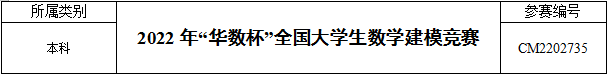
\includegraphics[scale=1]{figures/1.png} 基于神经网络的插层熔喷变量影响模型  }
\tihao{A}
\baominghao{}
\membera{ }
\memberb{ }
\memberc{ }
\supervisor{ }
\yearinput{2022}
\monthinput{07}
\dayinput{08}

\begin{document}

 \maketitle
 
 
 \begin{abstract}
插层熔喷法是通过在聚丙烯熔喷制备过程中将纤维插入熔喷纤维流,制备插层熔喷非织造材料,从而提高过滤效率的方法。插层熔喷非织造材料制备过程包括工艺参数、结构变量、产品性能三种指标。三种指标组内的变量以及指标之间的变量存在着交互影响,如果能够建立三种指标之间的关系模型,则有助于为调控插层熔喷非织造材料制备提供理论依据。


针对问题一:\textbf{第一步},通过绘制结构变量、产品性能插层前后与接受距离,热空气速度变化3D图,\textbf{定性}研究变量的变化规律\textbf{;}计算插层前后结构变量、产品性能变化的平均值和变化平均百分比,\textbf{定量}研究变量的变化规律,发现\textbf{插层后过滤阻力减小,剩余5个变量均变大}。\textbf{第二步},对插层前和插层后数据进行正态性检验和显著性检验,通过绘制插层前后结构变量、产品性能变化平均百分比随插层率的折线图,\textbf{定性}分析插层率对于这些变化的影响\textbf{;}计算插层率与插层前后结构变量、产品性能变化平均百分比的比尔森相关系数并进行相关性检验,\textbf{定量}分析插层率对于这些变化的影响,最终认为\textbf{插层率对于这些变化没有影响}。




针对问题二:通过搭建工艺参数到结构变量的神经网络并进行训练,间接得出工艺参数与结构变量的关系,并对8个工艺参数条件下的结构变量进行了预测。


针对问题三:\textbf{第一步},查看结构变量与产品性能的相关性系数矩阵,发现变量之间相关性较高,于是通过\textbf{典型相关分析},建立了结构变量与产品性能的关系模型。\textbf{第二步},分别对结构变量,产品性能之间的变量进行了\textbf{多元线性回归},建立了结构变量、产品性能变量之间的关系模型。\textbf{第三步},通过搭建工艺参数,结构变量到产品性能的神经网络并进行预测,得出\textbf{当接收距离为 23,热风速度为 1250 时,过滤效率达到最大,
为 66.38\%}。


针对问题四:将第二问和第三问的神经网络用数学公式进行表达并作为条件约束,建立并求解\textbf{线性规划}模型,得出结果:\textbf{当接收距离为 20.46cm, 热风距离为 1434.48(r/min), 厚度为 2.999mm, 孔隙率为 96.44\%,压缩回弹率为 26.13\% 时,过滤效率尽量的高的同时过滤阻力尽量的小 过滤效率为 94.977\% ,过滤阻力为 26.126\%}

\keywords{神经网络\quad  典型相关分析\quad   多元线性回归\quad  线性规划}
\end{abstract}

%目录  2019 明确不要目录,我觉得这个规定太好了
%\tableofcontents

%\newpage

\section{问题重述}
\subsection{问题背景}
插层熔喷法是通过在聚丙烯熔喷制备过程中将纤维插入熔喷纤维流,制备插层熔喷非织造材料,从而提高过滤效率的方法。插层熔喷非织造材料制备过程包括工艺参数、结构变量、产品性能三种指标。三种指标组内的变量以及指标之间的变量存在着交互影响,如果能够建立三种指标之间的关系模型,则有助于为调控插层熔喷非织造材料制备提供理论依据。

	
\subsection{具体问题}

\begin{enumerate}
	\item 根据插层前后数据,定性定量的研究插层后结构变量、产品性能的变化规律;定性定量的研究插层率对于这些变化是否有影响。
	\item 根据data3数据,建立工艺参数到结构变量的神经网络并进行预测
	\item 根据data3数据,建立结构变量到产品性能的神经网络
	\item 对结构变量和产品性能建立典型相关分析模型
	\item 对结构变量之间、产品性能之间建立多元线性回归模型
	\item 结合两个神经网络,求解最大效率下的工艺参数
	\item 根据神经网络模型和参数,写出过滤效率,过滤阻力与工艺参数的表达式,建立并求解线性规划模型,求出过滤效率尽量高、
过滤阻力尽量小时的工艺参数。
\end{enumerate}


\section{问题分析}
   针对问题一:data1与data2给出了插层前后结构变量、产品性能数据。为了探究插层前后的影响,首先需要对插层前和插层后的数据进行正态性检验,对插层前与插层后的数据进行显著性检验,然后通过绘制变化前后的图像查看变化趋势和情况并计算变化前后的平均值和平均变化百分比,从而分析结构变量、产品性能的变化规律。为了探究插层率的影响,可以对插层前后的数据进行差分,绘制变量随插层率变化的折线图,观察插层率大小对变量是否有影响,为了定量的探究插层率的影响,可以对差分后插层率对各个变量进行相关性检验,最终确定插层率对于这些变化是否有影响。
   
   
   针对问题二:问题二需要建立工艺参数与结构变量之间的关系模型,并且这种模型能够根据工艺参数给出结构变量结构。因此考虑神经网络,神经网络可以作为一种关系模型,并且轻量级的网络可以直接写出数学表达式,搭建神经网络之后即可进行数据预测。
   
   针对问题三:为了探究结构变量与产品性能的关系,可以考虑典型相关分析;结构变量、产品性能之间的关系可以考虑多元线性回归;求解过滤效率最高时的工艺参数,为了兼顾第二问与第四问,故搭建一个从结构变量到产品性能的神经网络从而进行预测与求解。
   
   
   针对问题四:可以将搭建的神经网络用数学公式进行表达并作为一个约束条件建立线性规划方程组进行求解。
   
   本文的论文研究思路如下:
   \begin{figure}[H]
   	\centering
   	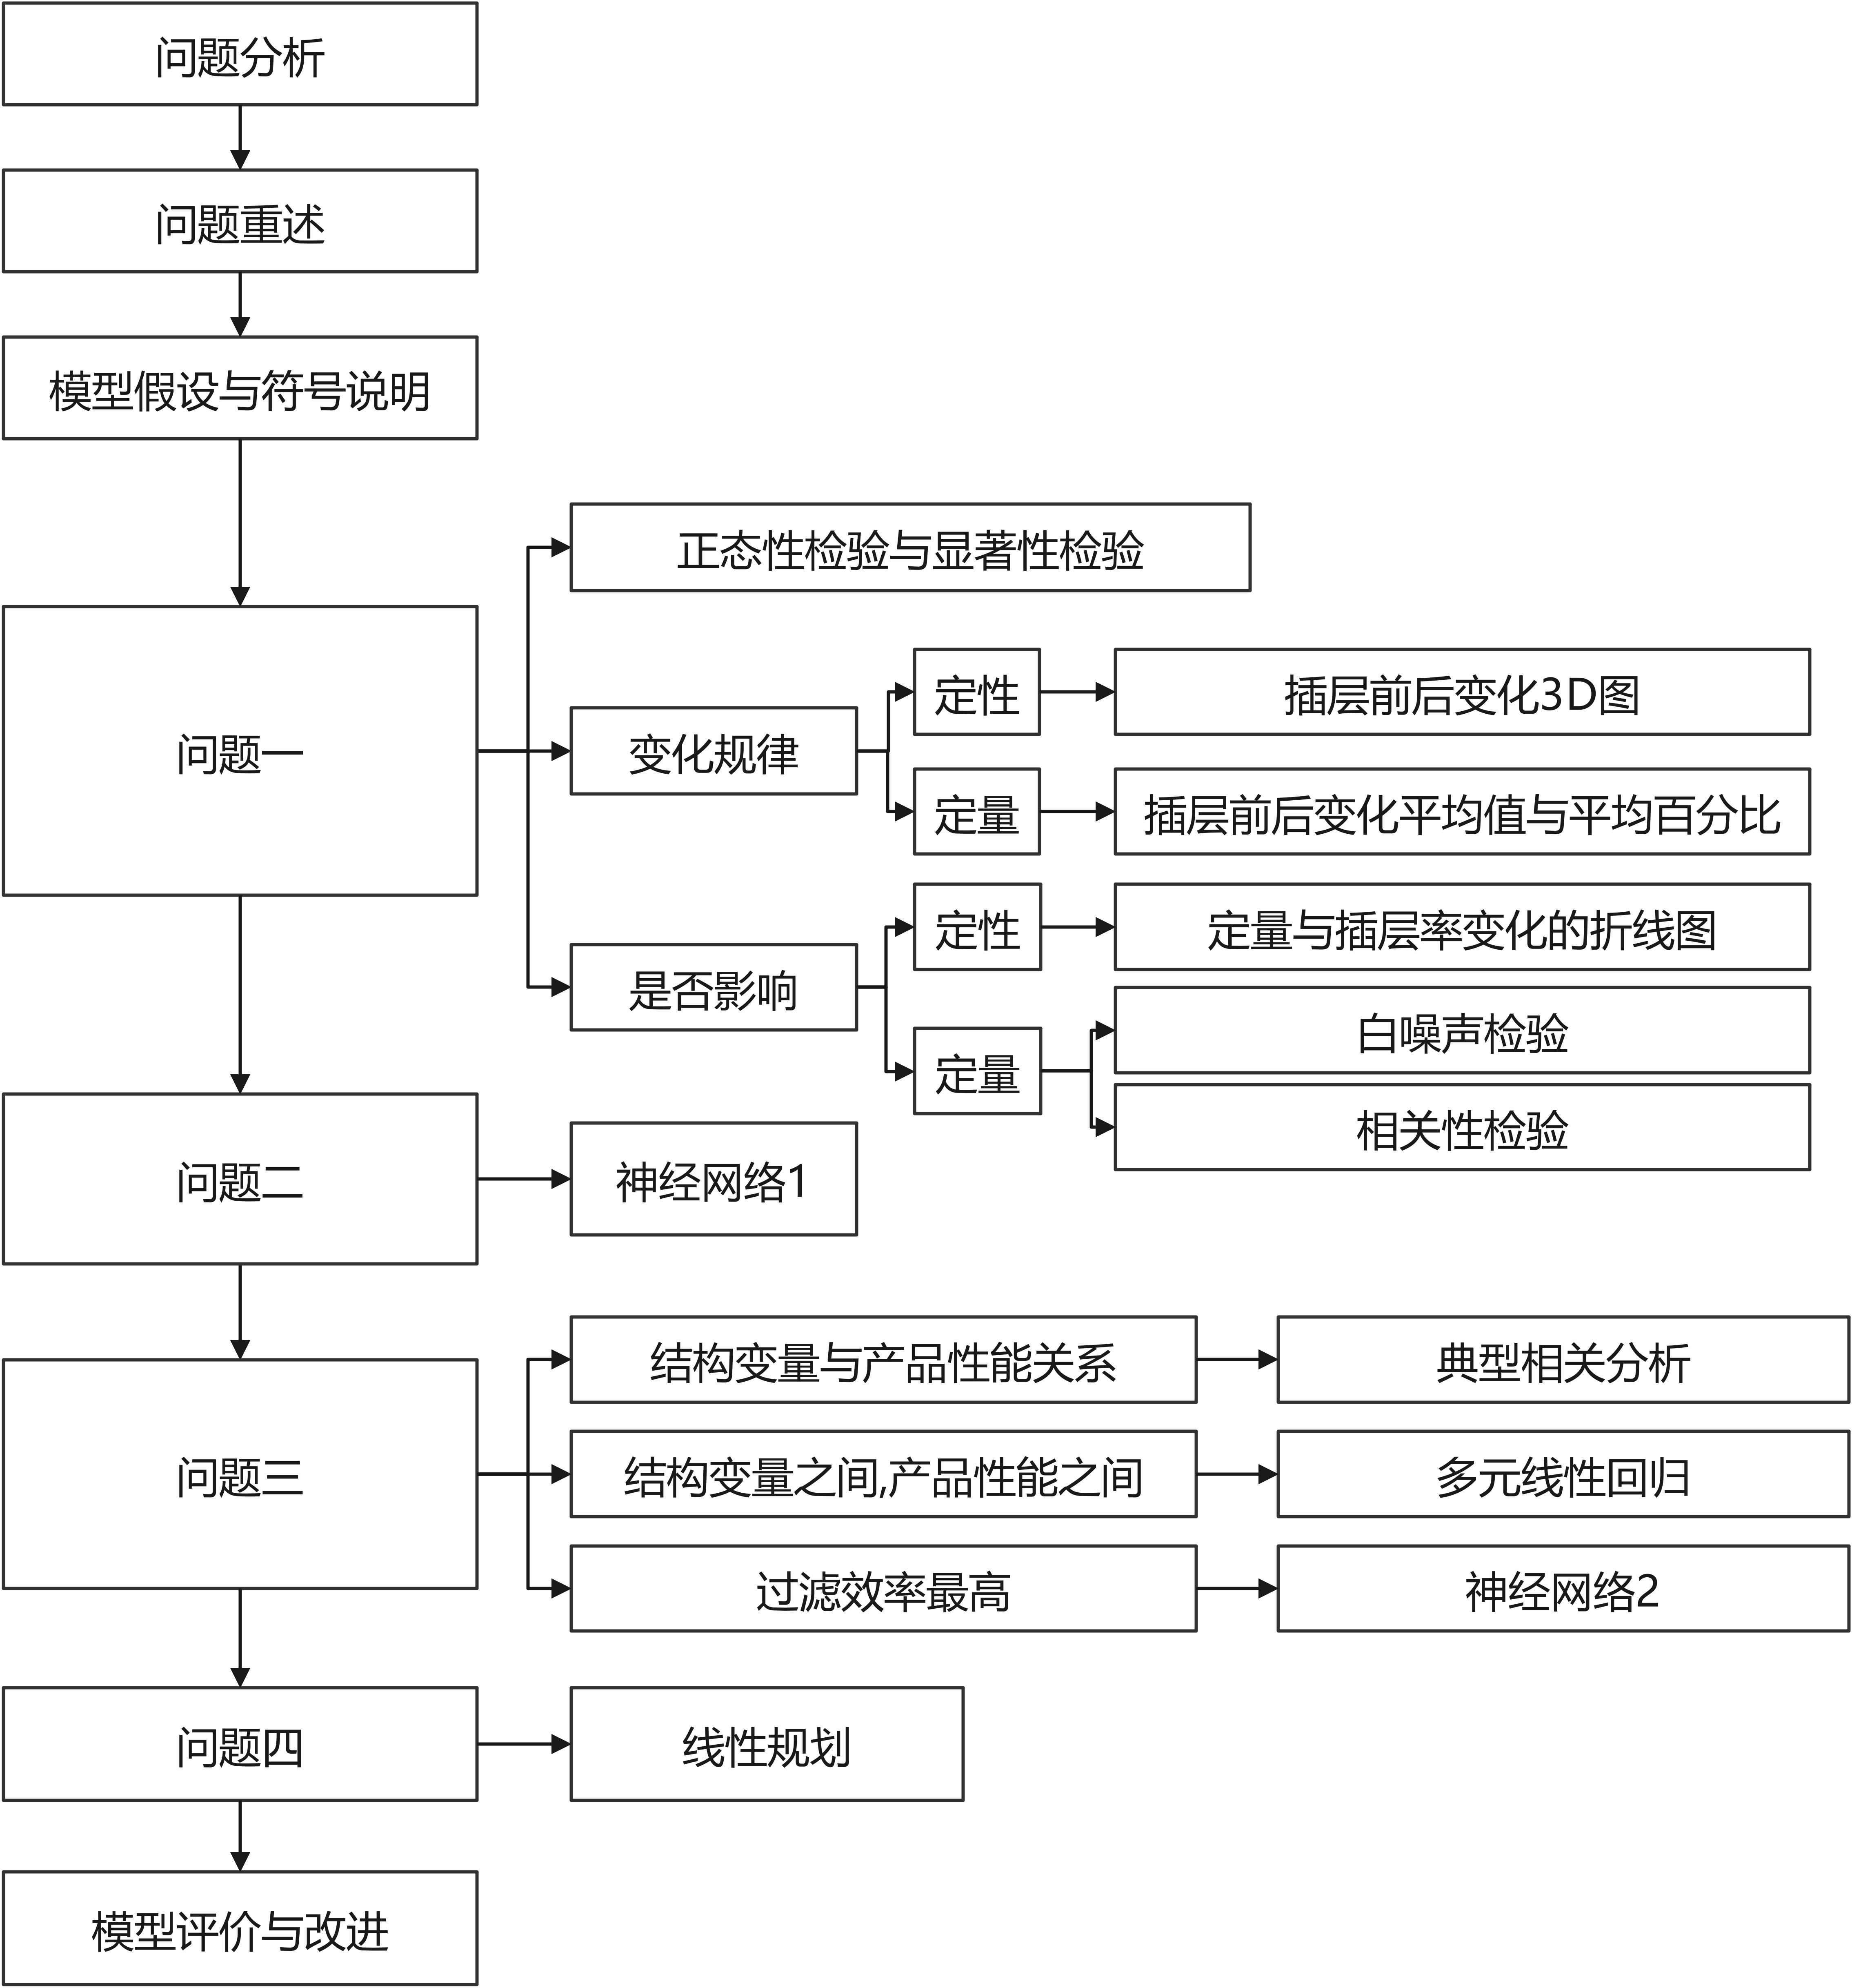
\includegraphics[scale=0.75,angle=0]{15.png}
   	\caption{论文思路图}
   	\label{2}
   \end{figure}
   
		
\section{模型假设}
\begin{enumerate}
	\item 假设结构变量之间,产品性能之间存在相互制约的影响关系
	\item 假设工艺参数决定结构变量,结构变量决定产品性能
	\item 假设工艺参数一定的情况下,结构变量的取值可以不同,但在一定的区间波动;同样的,工艺参数,结构变量一定的情况下,产品性能的取值可以不同,但在一定的区间内波动。
\end{enumerate}

\clearpage
\section{符号说明}
\begin{table}[h]
	\begin{center}
		\begin{tabular}{p{200pt}p{280pt}}
			\toprule
			符号    & 含义  \\
			\midrule
			$\{x_1,x_2\}$&工艺参数,分别代表接受距离和热空气速度 \\
			$\{y_1,y_2,y_3\}$&结构变量,分别代表厚度,孔隙率,压缩回弹性率 \\
			$\{z_1,z_2,z_3\}$&产品性能,分别代表过滤阻力, 过滤效率, 透气性 \\
			$A,B,\dots$     &   矩阵 \\
			$a_{ij}$ & 矩阵A中的第i行第j列的元素   \\	
			$\sum$  &  求和符号 \\
			$\frac{\partial G}{\partial a}$  &  求$G$关于$a$的偏导数    \\	
			$ g_1 (x_1 ,x_2 ),f_1 (y_1 ,y_2 ,y_3 )$    &   多元函数   \\
			
			
			
			
			\bottomrule
		\end{tabular}
	\end{center}
\end{table}

\section{问题一模型的建立与求解}
\subsection{正态性检验与显著性检验}
为了探究插层前后的影响,首先需要对插层前和插层后的数据进行正态性检验,对插层前与插层后的数据进行显著性检验。
\subsubsection{数据预处理}
本文用到的数据预处理主要包括三个方面:在data1中添加两列,填充每组实验下data2中对应的工艺参数;将插层前的数据与插层后的数据进行分离,进行正态性检验和显著性检验;对插层后的数据和插层前的数据进行差分。
\subsubsection{正态性检验}
对插层前和插层后的数据进行正态性检验,检验结果如下:
   \begin{figure}[H]
	\centering
	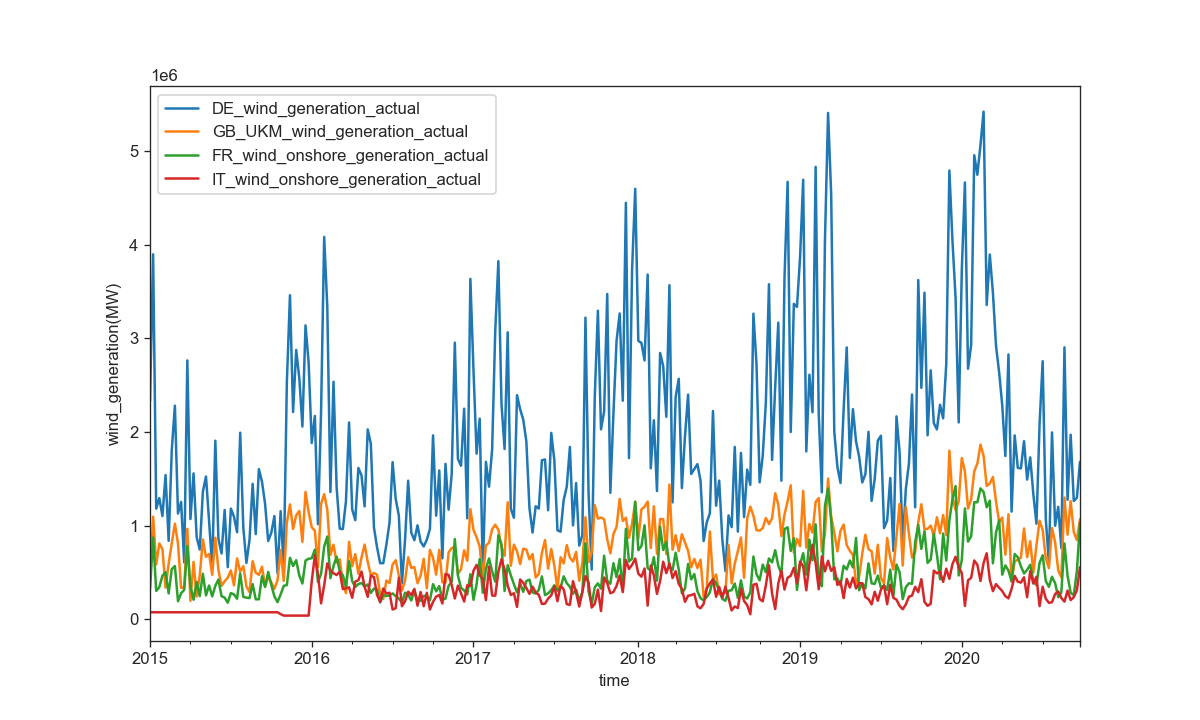
\includegraphics[scale=0.5,angle=0]{2.png}
	\caption{正态性检验}
	\label{2}
\end{figure}
从以上的结果可以看出,无论是插层前还是插层后,$p$值的数量级已经达到了$10^{-18}$,数据具有优良的正态分布特性。

\subsubsection{显著性检验}
对插层前和插层后的数据进行显著性检验,检验结果如下:
\begin{figure}[H]
	\centering
	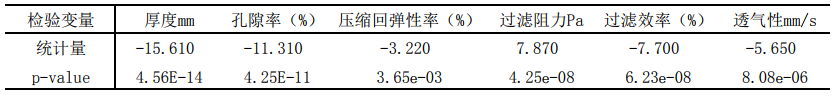
\includegraphics[scale=0.8,angle=0]{3.png}
	\caption{显著性检验}
	\label{3}
\end{figure}
从以上的结果可以看出,6个变量的$p$值均小于$0.01$,结构变量在插层前后具有明显的差异,显著性检验通过。

\subsection{结构变量、产品性能变化规律}
通过插层前后的数据,绘制结构变量、产品性能3D变化图如下:
   \begin{figure}[H]
	\centering
	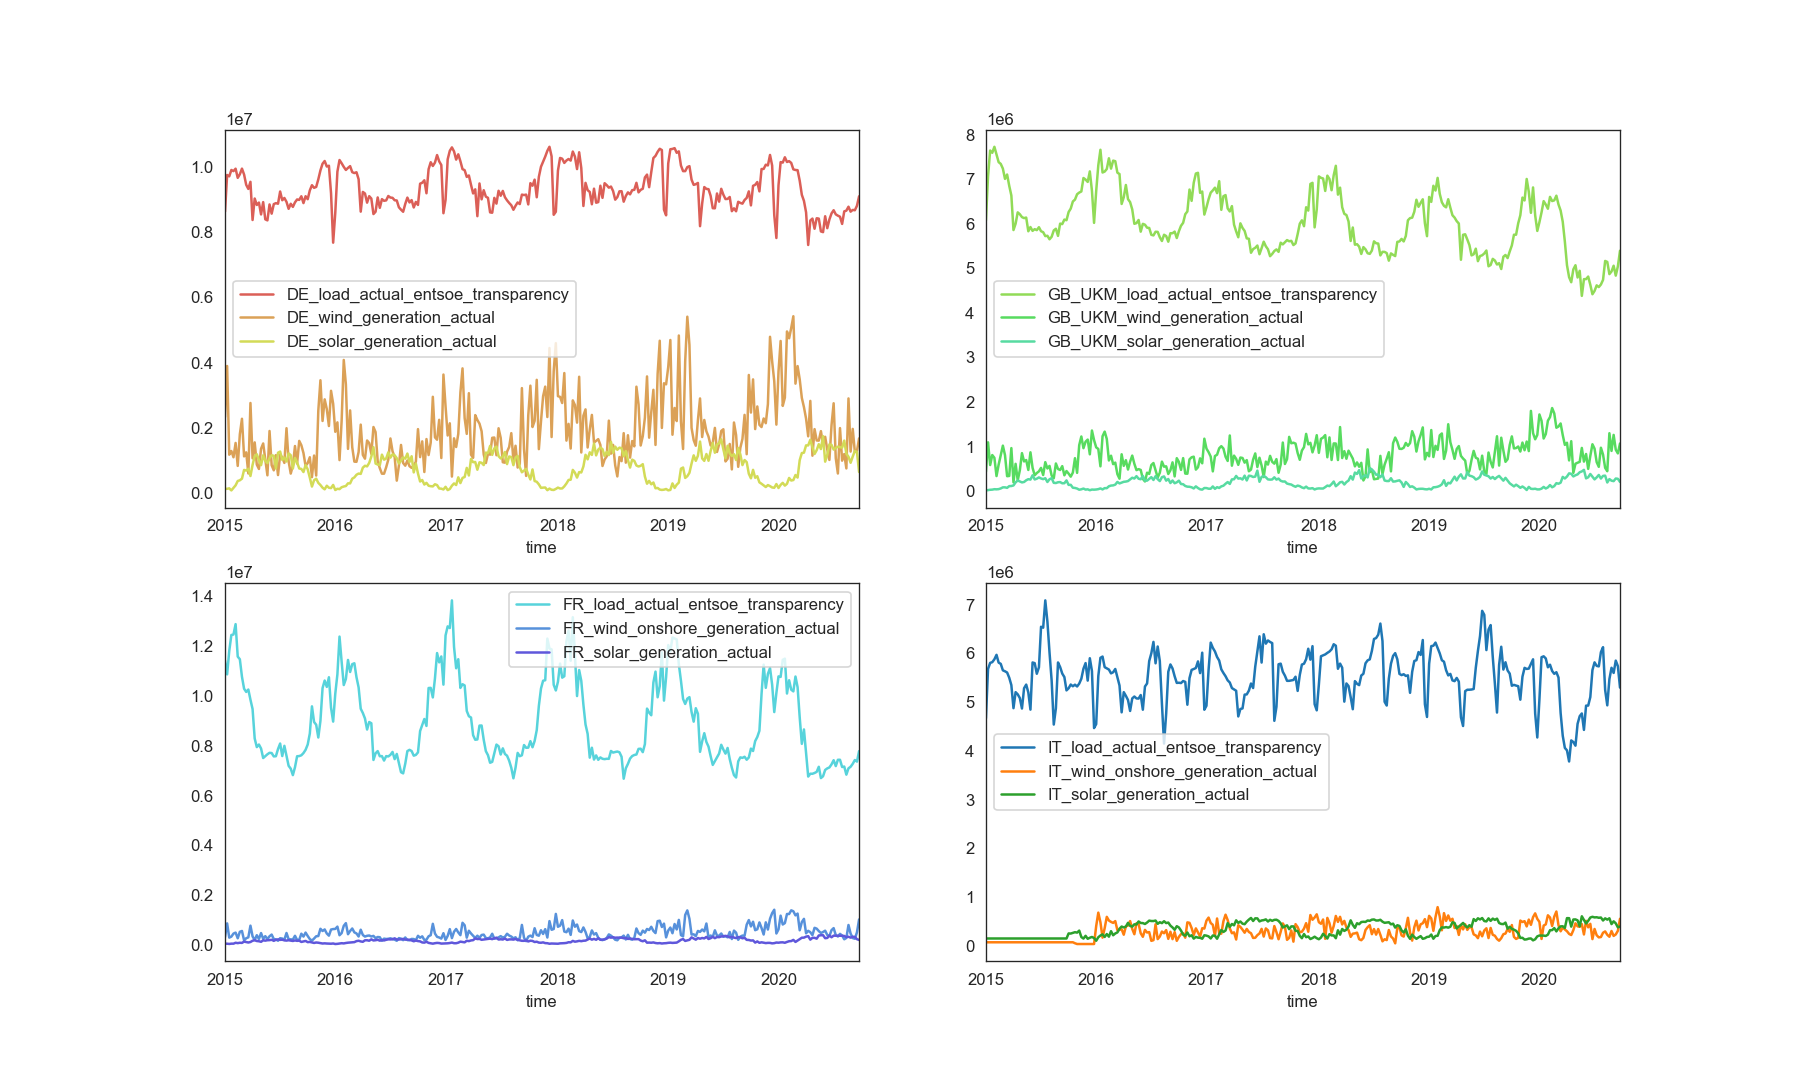
\includegraphics[scale=0.45,angle=0]{4.png}
	\caption{结构变量、产品性能变化3D图}
	\label{5}
\end{figure}
从图中可以得到以下结论:

\begin{itemize}
\item 插层后的厚度均比插层前大,并且厚度随接受距离的增加而增加,随热风速度的增大而增大;
\item 插层后的孔隙率均比插层前大,并且孔隙率随热风速度的增加而增加,随接受距离的增加出现先上升后下降再上升的趋势;
\item 插层后的压缩回弹性率大部分比插层前大,少部分比插层前小,并且压缩回弹性率随接收距离的增加出现先上升后下降的趋势,随热风速度的增加出现先上升后下降的趋势;
\item 插层后的过滤阻率均比插层前小,并且过滤阻力随接受距离的增加而减小,随热风速度的增加而增大;
\item 插层后的过滤效率均比插层前大,并且过滤效率随接收距离的增加而减小,随热风速度的增加而增加;
\item 插层后的透气性均比插层前大,并且透气性随热风速度的增加而减小,随接受距离的增加而增加。
\end{itemize}

计算插层前后结构变量、产品性能变化平均值和变化平均百分比,得到结果如下:
   \begin{figure}[H]
	\centering
	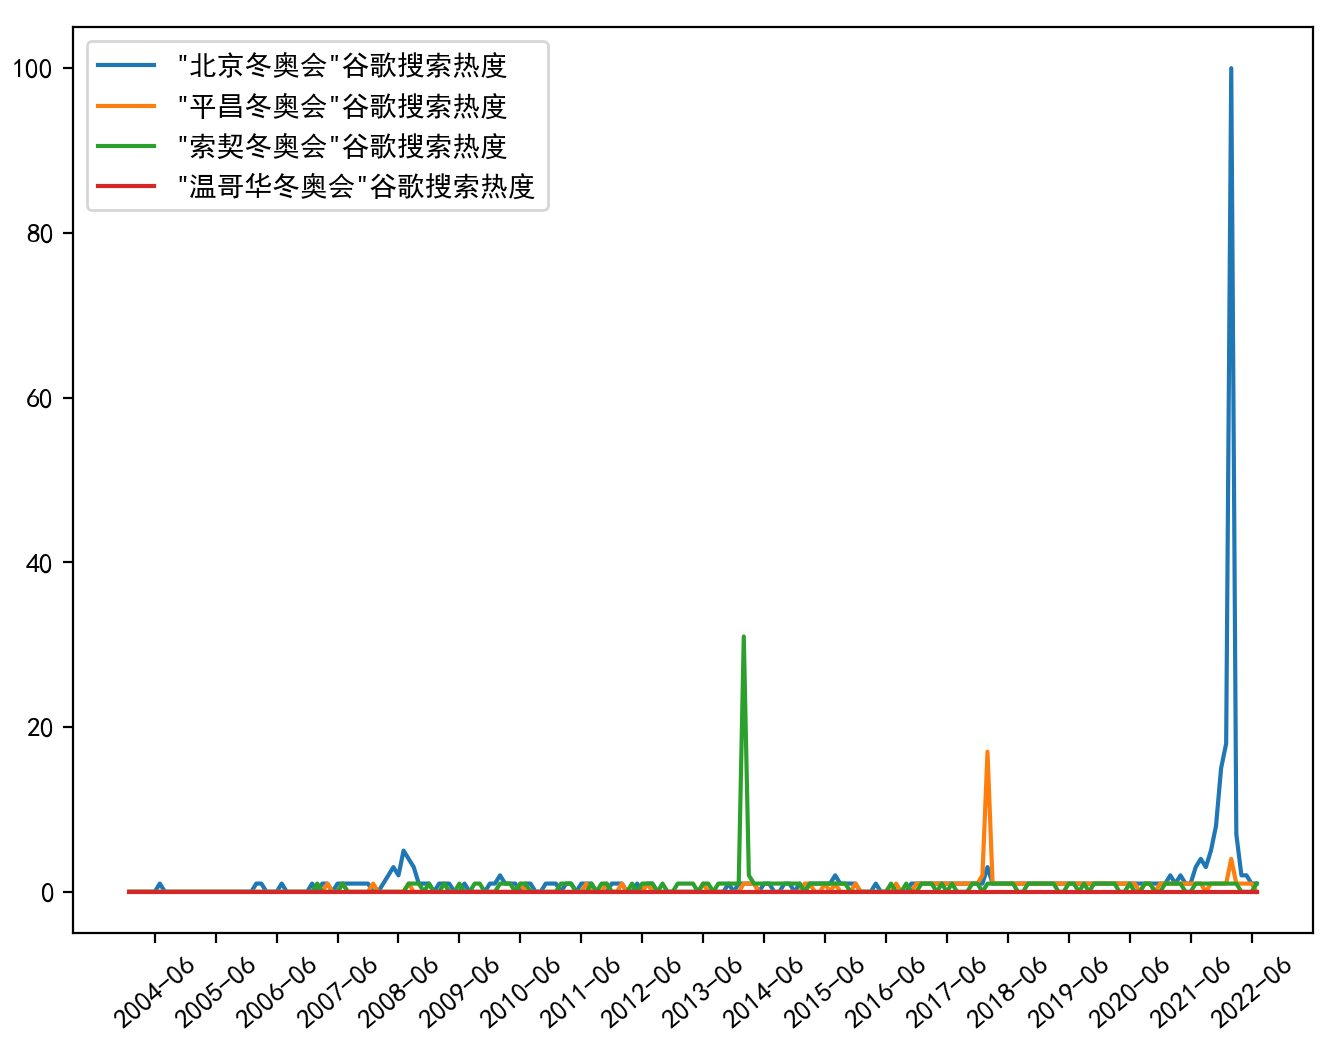
\includegraphics[scale=0.8,angle=0]{5.png}
	\caption{结构变量、产品性能插层前后变化}
	\label{6}
\end{figure}
从计算结果可以看出插层后厚度、压缩回弹性、过滤效率、透气性均有显著提升,孔隙率有所提升,而过滤阻力则有显著下降。


\subsection{插层率影响}
对差分后的数据按插层率进行排序,绘制各变量随插层率从小变大的变化图如下:
   \begin{figure}[H]
	\centering
	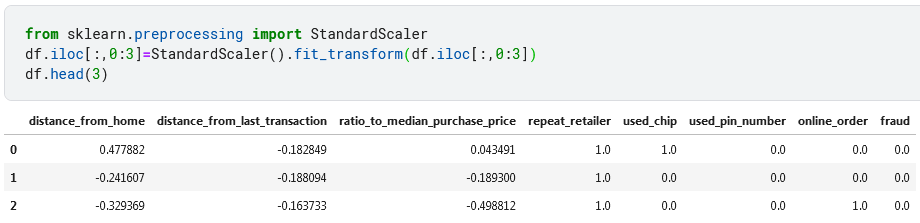
\includegraphics[scale=0.31,angle=0]{7.png}	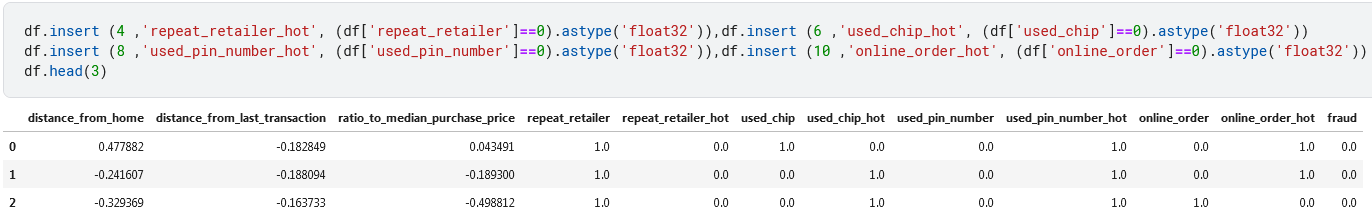
\includegraphics[scale=0.31,angle=0]{8.png}
	\caption{结构变量、产品性能与插层率折线图}
	\label{78}
\end{figure}
从图中可以看出六个量随插层率的增加的变化无规律可循,对数据进行随机性检验,检验结果如下:
   \begin{figure}[H]
	\centering
	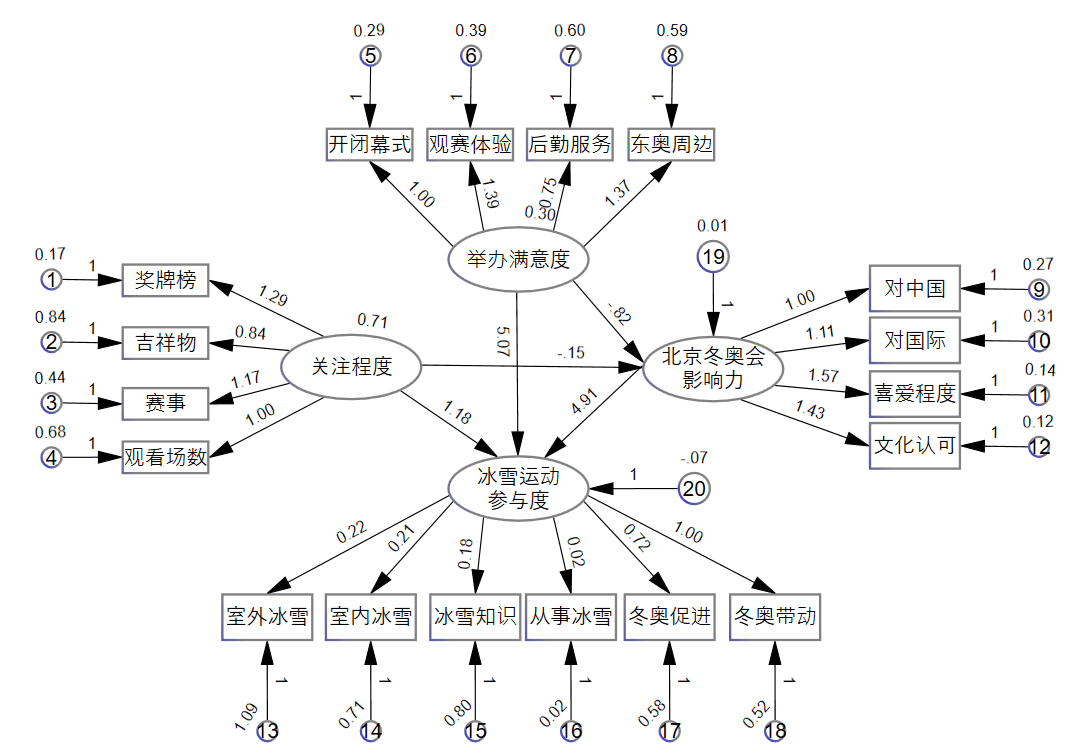
\includegraphics[scale=0.8,angle=0]{9.png}	
	\caption{随机性检验}
	\label{8}
\end{figure}
从检验结果可以看出,$p$的值均大于0.01,可以认定为白噪声,即插层率对6个变量没有影响。

对属性插层率和6个变量的进行相关性检验,检验结果如下:
   \begin{figure}[H]
	\centering
	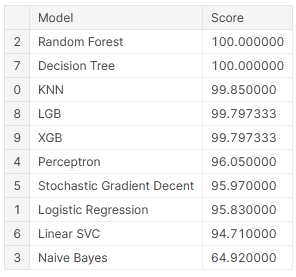
\includegraphics[scale=0.8,angle=0]{10.png}	
	\caption{相关性检验}
	\label{9}
\end{figure}
从检验结果来看,插层率与6个变量的相关性均比较小,并且p值均大于0.05,可以认为插层率对6个变量没有影响。




\section{问题二模型的建立与求解}
\subsection{神经网络}
神经网络是一种模仿动物神经元而产生的模型,可用于分类,回归等问题,模型效果良好。神经网络在理论上能够拟合任意函数,包括非线性函数,是当下最流行的数学建模方法之一。

1959年两个生物科学家发现青蛙的神经元接受多个输入,输入包括青蛙的多个器官的输入,只有单输入的和到达一个阈值,才会有输出(青蛙接受的刺激比较大时才会有反应。)
于是计算机科学家仿照生物神经元的原理和结构,提出了感知器,感知器可以表示为$$y=o(\sum_{i=0}^{n} w_{i} x_{i}+w_0),$$其中

$$	o(x)=\left\{\begin{array}{c}
x ,~~~~x>0 \\
0, ~~~~x \leq 0
\end{array}\right.
$$
\begin{figure}[H]
	\centering
	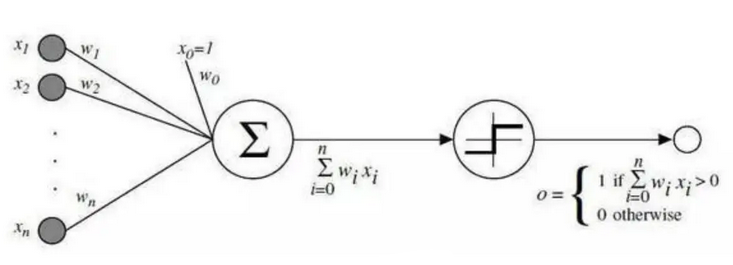
\includegraphics[scale=0.45,angle=0]{93.png}
	\caption{感知器}
	\label{93}
\end{figure}
在感知器的基础上,科学家们设置了输入层,隐藏层,输出层,并在每一层设置若干个感知器,形成了神经网络。
\begin{figure}[h]
	\centering
	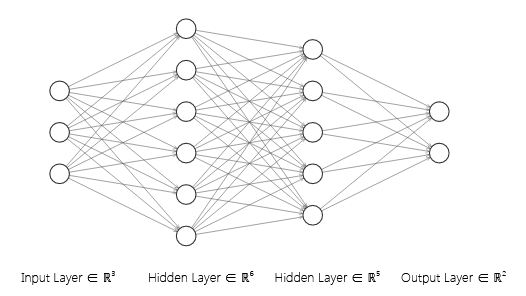
\includegraphics[scale=0.75,angle=0]{94.png}
	\caption{神经网络}
	\label{94}
\end{figure}
神经网络使用梯度下降法求解最优值,梯度下降法是一类求解函数最小值的计算机算法。假设希望求解目标函数 
$ f(x)=f(x_1,\dots ,x_n) $的最小值,可以从一个初始点 $ x^{(0)}=(x_1^{(0)},\dots ,x_n^{(0)}) $开始,基于学习率 $\alpha > 0$ 构建一个迭代过程:\begin{gather*}
x_1^{i+1}=x_1^{i}+\alpha \frac{\partial f}{\partial x_1}(x^{(i)})\\
\vdots \\
x_1^{i+1}=x_1^{i}+\alpha \frac{\partial f}{\partial x_1}(x^{(i)})
\end{gather*}	 其中$x^{(i)}=(x_1^{(i),\dots,x_n^{(n)}}),i>=0$,一旦达到收敛条件的话,迭代就结束了。图\ref{5}是用剃度下降法求解$y=x^2$的最小值时迭代10次的过程,其中的点代表每次迭代后的值。
\begin{figure}[h]
	\centering
	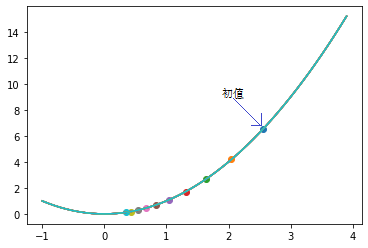
\includegraphics[scale=0.7,angle=0]{95.png}
	\caption{剃度下降法图解}
	\label{95}
\end{figure}


\subsection{网络一搭建与预测}
\subsubsection{网络一设置}
神经网络的输入为接受距离与热风速度,输出为厚度,孔隙率,压缩回弹性率。具体的神经网络结构如下:
   \begin{figure}[H]
	\centering
	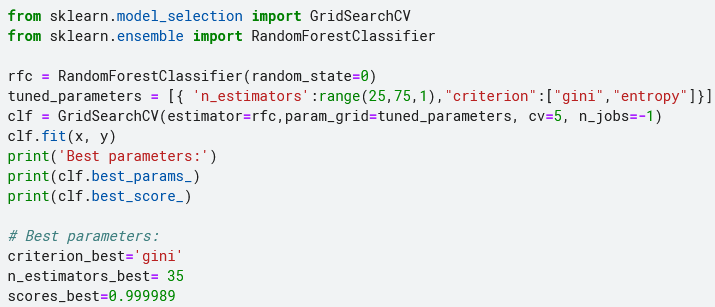
\includegraphics[scale=0.25,angle=0]{11.png}	
	\caption{网络1结构}
	\label{11}
\end{figure}
网络一的激活函数为$Softplus$,数学表达式为:$$f(x)=\frac{1}{\beta}ln(1+e^{\beta x}),$$ 
其中$\beta$为常数,$x$为上一层网络的输出。网络1的损失函数为均方差损失函数$$loss=\sum_{k=1}^{n} \sum_{i=1}^m(f(x_i)-y_i)^2,$$其中$k$为神经网络输出变量的个数。$f(x_i),y_i$分别代表网络的预测值和真实值。数据集为data3中的所有数据,训练集与测试集比例为$8:2$,采取随机抽取方式。
\subsubsection{网络训练}
对神经网络进行训练,在测试集上损失值得变化如下:
   \begin{figure}[H]
	\centering
	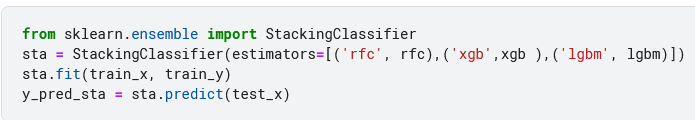
\includegraphics[scale=0.3,angle=0]{13.png}	
	\caption{问题二预测结果}
	\label{11}
\end{figure}

\subsubsection{网络预测}
通过训练好的神经网络对问题二给出的数据进行预测,得到预测结果如下:
   \begin{figure}[H]
	\centering
	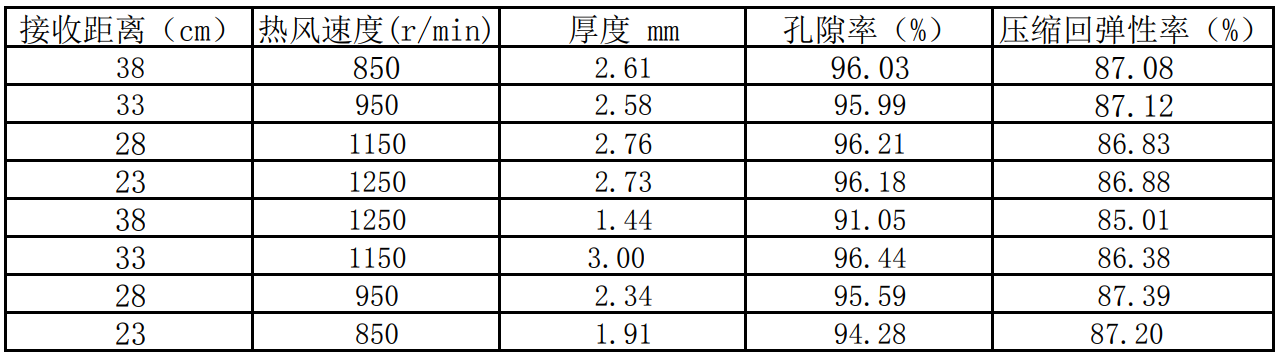
\includegraphics[scale=0.5,angle=0]{12.png}	
	\caption{问题二预测结果}
	\label{11}
\end{figure}


\section{问题三模型的建立与求解}
\subsection{结构变量与产品性能的关系}
计算结构变量与产品性能之间的相关系数矩阵如下:
   \begin{figure}[H]
	\centering
	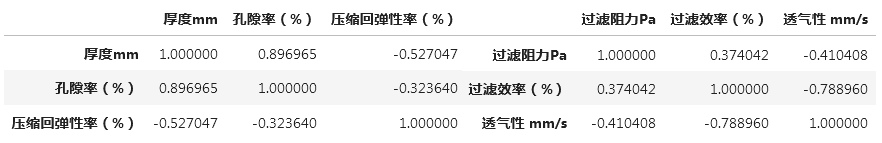
\includegraphics[scale=0.71,angle=0]{14.png}	
	\caption{结构变量,产品性能相关系数矩阵}
	\label{11}
\end{figure}
发现组内变量均有相关性,为了探究结构变量与产品性能的关系,考虑构建典型相关分析模型。典型相关分析是探究两组变量之间相关性的模型,假设结构变量为$y_1,y_2,y_3$,分别代表厚度,孔隙率,压缩回弹性率;产品性能为$z_1,z_2,z_3$,分别代表过滤阻力Pa,过滤效率, 透气性。设随机向量 $$ y=\left(Y_{1}, Y_{2} , Y_{3}\right)^{\prime}, z=\left(Z_{1}, Z_{2}, Z_{3}\right)^{\prime} ,$$
y, z  的协方差阵为:
$$\operatorname{cov}\left[\begin{array}{l}
	y \\
	z
\end{array}\right]=\Sigma=\left[\begin{array}{ll}
	\Sigma_{11} & \Sigma_{12} \\
	\Sigma_{21} & \Sigma_{22}
\end{array}\right]$$
为了研究两组变量之间的相关关系, 列出它们的 线性组合:
$$\begin{array}{l}
	\mu_{1}=a^{\prime} y=a_{11} Y_{1}+a_{12} Y_{2}+a_{1 3} Y_{3} \\
	v_{1}=b^{\prime} z=b_{11} Z_{1}+b_{12} Z_{2}+b_{1 3} Z_{3}
\end{array}$$
求出  $\mu_{1}$  与  $v_{1}$  之间的相关系数:
$$\rho=\frac{\operatorname{cov}\left(\mu_{1}, v_{1}\right)}{\sqrt{\operatorname{var}\left(\mu_{1}\right) \operatorname{var}\left(v_{1}\right)}}=\frac{\operatorname{cov}\left(a^{\prime} y, b^{\prime} z\right)}{\sqrt{\operatorname{var}\left(a^{\prime} y\right) \operatorname{var}(b z)}} $$
令  $\mu_{1}$, $v_{1}$  的方差为$ 1$ , 可得 $ \rho=a^{\prime} \sum_{12} b $ 。运用拉 格朗日乘数法将问题等价为:
$$G=a^{\prime} \sum_{12} b-\frac{\lambda}{2}\left(a^{\prime} \sum_{11} a-1\right)-\frac{\mu}{2}\left(b \sum_{22} b-1\right)$$
上式 分别对求偏导并令其等于 0 , 得:
$$\left\{\begin{array}{l}
	\frac{\partial G}{\partial a}=\Sigma_{12} b-\lambda \Sigma_{11} a=0 \\
	\frac{\partial G}{\partial b}=\Sigma_{21} a-\mu \Sigma_{22} b=0
\end{array}\right.
$$
$\text{用} a^{\prime},b^{\prime} \text{分别左乘上式,推出} \mu=b^{\prime} \sum_{21} a=\left(a^{\prime} \sum_{12} b\right)=\lambda$, 因此上式 可转化为:
$$\left\{\begin{array}{l}
	\Sigma_{12} b-\lambda \Sigma_{11} a=0 \\
	\Sigma_{21} a-\lambda \Sigma_{22} b=0
\end{array}\right.$$
通过软件求解得到:
$$\mu = 0.990y_1-0.018y_2+0.141y_3$$
$$ v  =-0.743z_1-0.553z_2-0.348z_3$$
$$\mu=0.884v$$
\subsection{结构变量之间,产品性能之间的关系}
为了表示结构变量之间,产品性能之间的关系,建立多元线性回归模型。设
$$y_1=\alpha_1 y_2 + \alpha_2 y_3+b_1$$
$$z_2=\beta_1 z_1 + \beta_2 z_3+b_2$$
求解得:
$$y_1=0.467 y_2 -0.103 y_3-33.293$$
$$z_2=0.141 z_1 -0.096 z_3+89.782$$

\subsection{过滤效率最高时的工艺参数}
为了求解过滤效率最高时的工艺参数,构建一个新的神经网络,输入为接受距离,热风速度,厚度,孔隙率,压缩回弹性率,输出为过滤阻力或者过滤效率其中一个。
具体的神经网络结构如下:
	\begin{figure}[H]
		\centering
		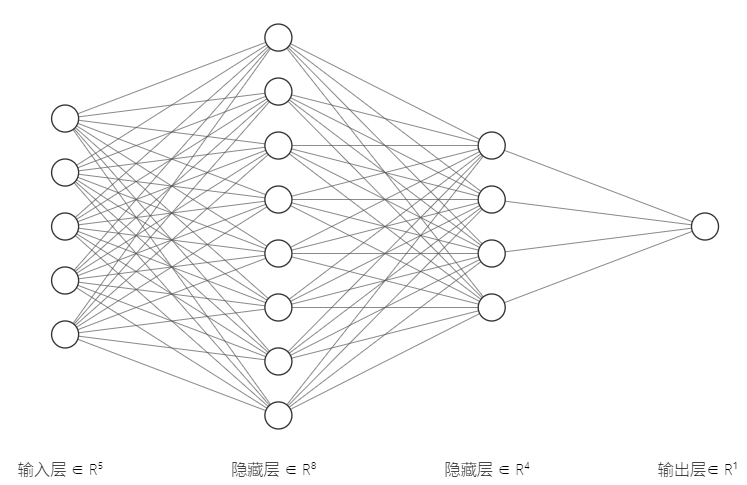
\includegraphics[scale=0.5,angle=0]{17.png}	
		\caption{网络2结构}
		\label{17}
	\end{figure}
	网络2的激活函数为$Relu$,数学表达式为:
	$$	f(x)=\left\{\begin{array}{c}
	x ,~~~~x>0 \\
	0, ~~~~x \leq 0
	\end{array}\right.
	$$
其中$x$为上一层网络的输出。网络2的损失函数为均方差损失函数$$E= \sum_{i=1}^m(f(x_i)-y_i)^2,$$$f(x_i),y_i$分别代表网络的预测值和真实值。数据集为data3中的所有数据,训练集与测试集比例为$8:2$,采取随机抽取方式。对网络进行训练,将问题二的表格作为输入,通过神经网络模型2可以得到:
	\begin{figure}[H]
	\centering
	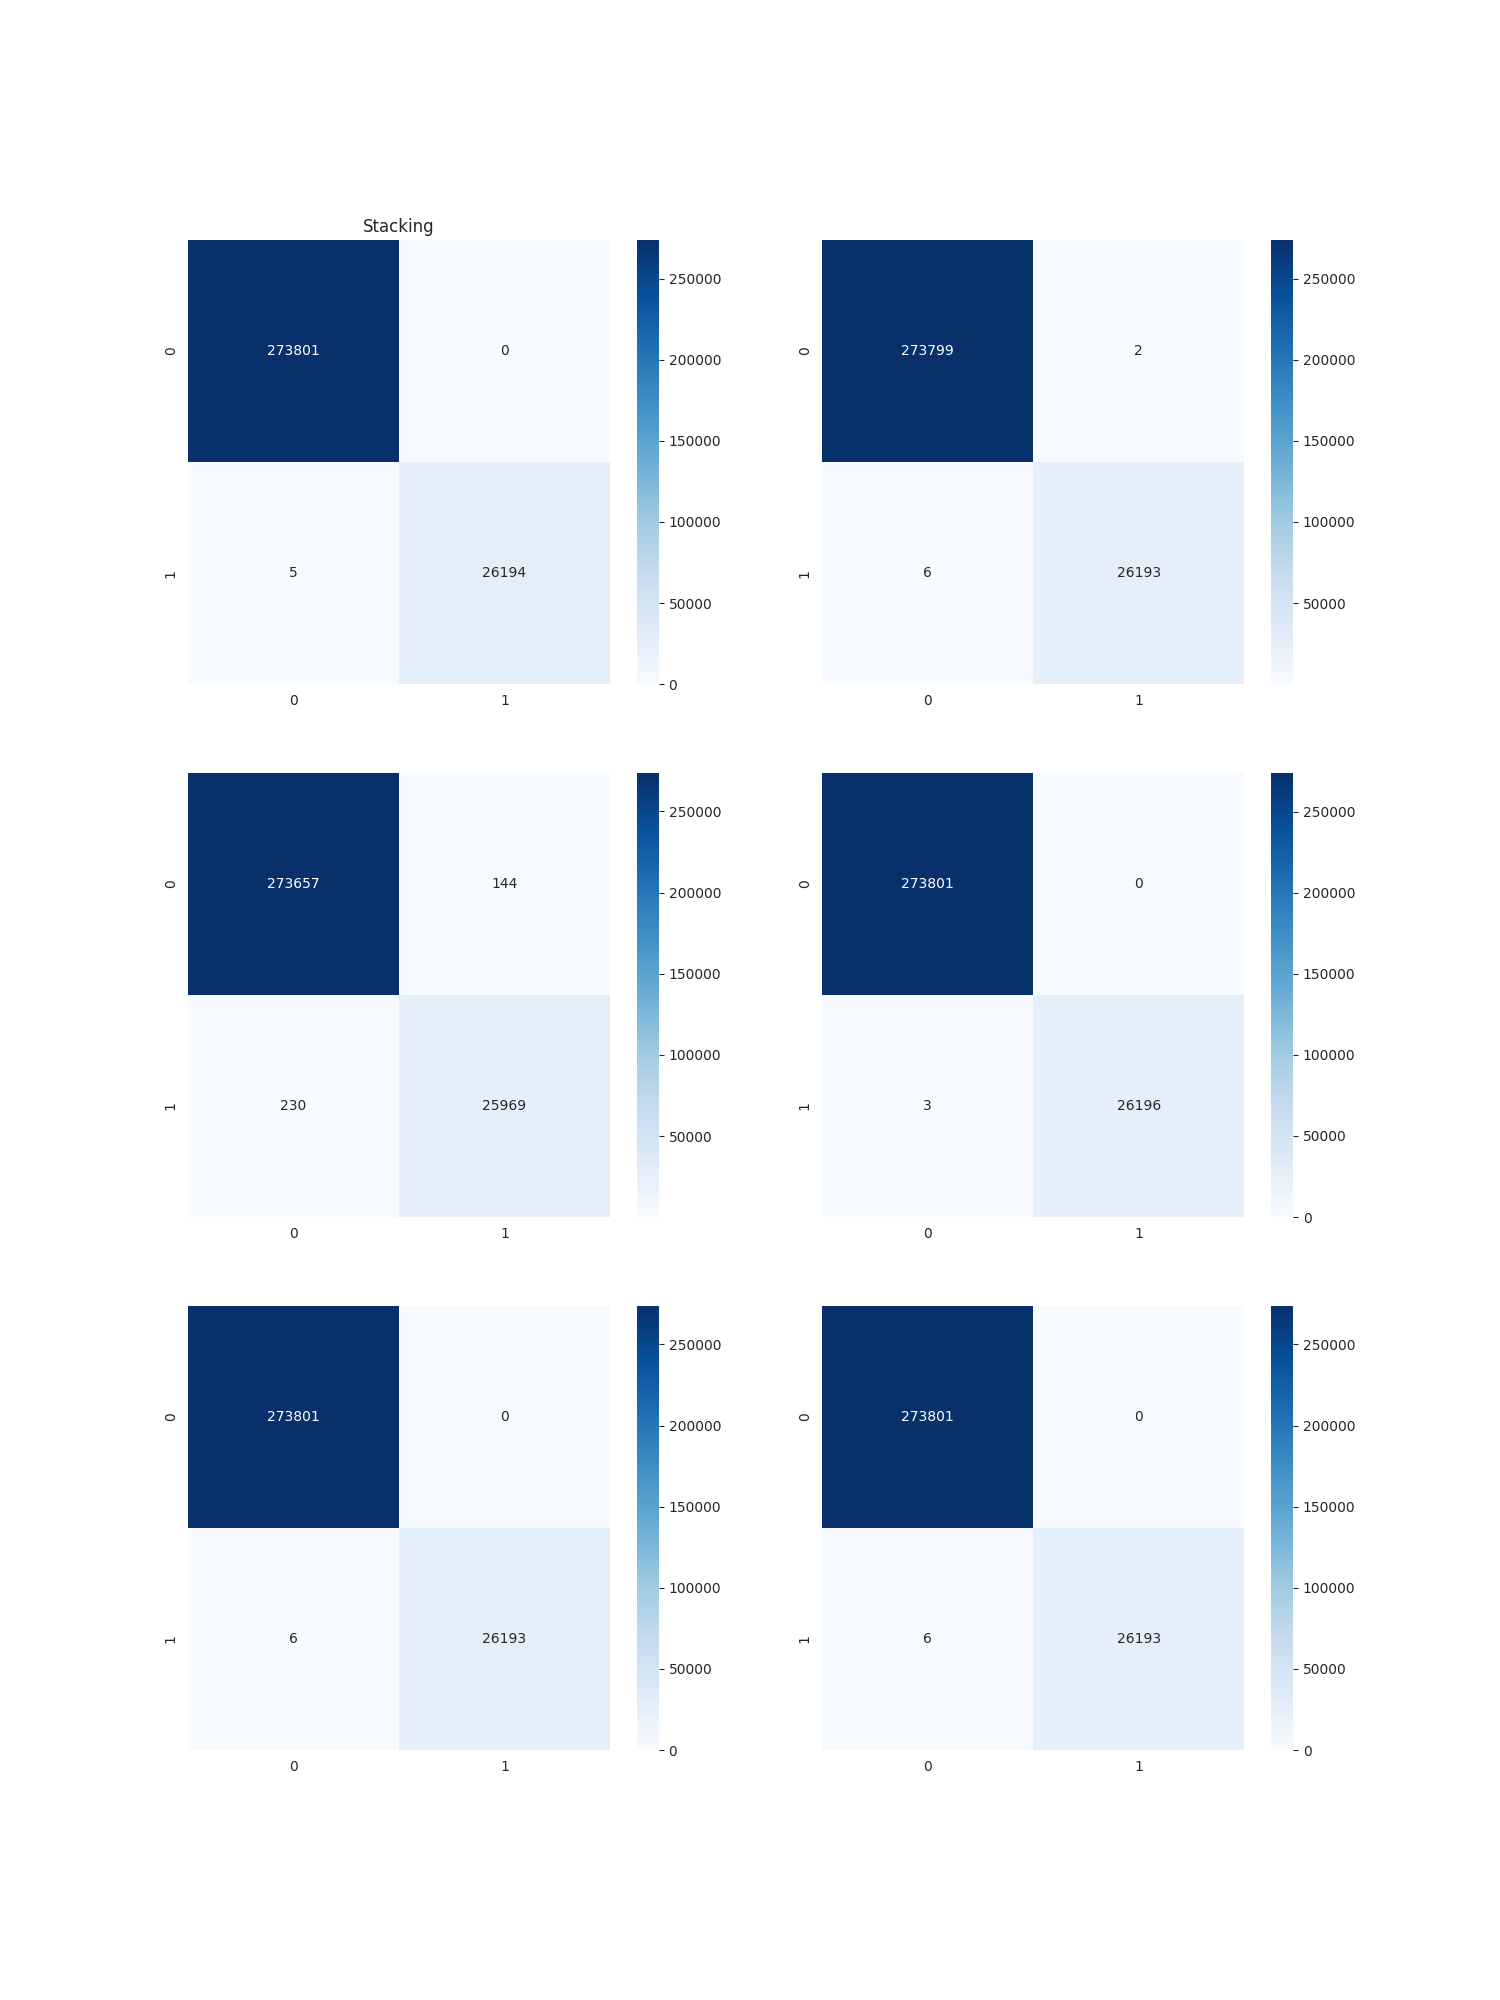
\includegraphics[scale=0.75,angle=0]{16.png}	
	\caption{预测结果}
	\label{16}
\end{figure}
从预测结果可以看出,\textbf{当接受距离为23,热风速度为1250时,过滤效率达到最大,为66.38\%}。
	
	
\section{问题四模型的建立与求解}	
神经网络可以认为是函数的集合,只要获取神经网络的权重参数以及激活函数,就可以写出每一个输出变量关于输入变量的函数关系式。根据神经网络2,$z_1,z_2$是关于$y_1,y_2,y_3$的函数即:
$$z_1=f_1(y_1,y_2,y_3),$$
$$z_2=f_2(y_1,y_2,y_3),$$
而神经网络1是$y_1,y_2,y_3$关于$x_1,x_2$的函数集合,即:
$$y_1=h_1(x_1,x_2),$$
$$y_2=h_2(x_1,x_2),$$
$$y_3=h_3(x_1,x_2),$$
因此$z_1,z_2$是关于$x_1,x_2$的函数,我们设为
$$z_1=g_1(x_1,x_2),$$
$$z_2=g_2(x_1,x_2)$$
根据问题四的条件,建立线性规划模型如下:
$$\begin{array}{c}
\max  w=\mathrm{g}_{2}\left(x_{1}, x_{2}\right)-\mathrm{g}_{1}\left(x_{1}, x_{2}\right) \\
\left\{\begin{array}{c}
\mathrm{x}_{1} \leq 100 \\
\mathrm{x}_{2} \leq 2000 \\
\mathrm{~h}_{1}\left(\mathrm{x}_{1}, \mathrm{x}_{2}\right) \leq 3 \\
\mathrm{~h}_{3}\left(\mathrm{x}_{1}, \mathrm{x}_{2}\right) \geq 0.83 \\
\mathrm{~g}_{2}\left(\mathrm{x}_{1}, \mathrm{x}_{2}\right) \geq 90 \\
\mathrm{~g}_{1}\left(\mathrm{x}_{1}, \mathrm{x}_{2}\right) \leq 26.5 \\
\mathrm{x}_{1}, \mathrm{x}_{2} \geq 0
\end{array}\right.
\end{array}$$
其中$g_2(x_1,x_2)$,为过滤效率,为了使过滤效率具有较高的值,我们增加约束条件$g_2(x_1,x_2)>90$;$g_1(x_1,x_2)$为过滤阻力,为了使过滤效率小,我们增加了约束条件$g_1(x_1,x_2)<=26.5$,该方程理论上是有解的,但局限于笔者的能力,最终使用了计算机的遍历求解算法,在上述约束条件下,求得最优解为
$$[x_1,x_2,y_1,y_2,y_3,z_1,z_2]=\left[\begin{array}{lllllll}
20.460 & 1434.482 & 2.999 & 96.438 & 86.381 & 26.126 & 94.977
\end{array}\right]
$$

因此当接受距离为20.46,热风距离为1434.48,厚度为2.999mm,孔隙率为96.44\%,压缩回弹率为26.13时,过滤效率高达94.977\%而过滤阻力低至26.126\%,过滤效率高而过滤阻力小。

	
	
	
	
	
	
	
	
	
		
	
	
\section{模型的评价及优化}
\subsection{优点}
\begin{enumerate}
	\item  \textbf{定性分析与定量计算结合}。针对问题一,研究变量变化规律,采用定性分析与定量计算的方式;研究插层率,采用定型分析与定量计算的方式,是模型更具有说服力。
	
	\item \textbf{更好的预测效果}神经网络相对于其他模型有更好的拟合能力和预测效果。
	

\end{enumerate}

\subsection{缺点}
\begin{enumerate}
	\item 神经网络的预测具有局限性,对于数据域在训练样本意外的数据,网络的误差会更大。
\end{enumerate}
\subsection{模型的改进}
\begin{enumerate}
	\item 优化神经网络结构,获取更优的模型效果。
	\item 求data3数据平均值,进行数据增强。
	\item 对数据进行标准化,归一化。
\end{enumerate}


\begin{thebibliography}{9}%宽度9
    \bibitem{1}朱婉宁,卢媛.四川省经济发展水平与旅游发展水平典型相关分析[J].绿色科技,2022,24(07):215-218+222.
\end{thebibliography}

\newpage
%附录


\end{document} 